% Chapter Template

\chapter{Introduction} % Main chapter title

\label{ChapterX} % Change X to a consecutive number; for referencing this chapter elsewhere, use \ref{ChapterX}

%----------------------------------------------------------------------------------------
%	SECTION 1
%----------------------------------------------------------------------------------------

Let us imagine a science fiction. Astronauts are coming back from World 2.0 after successfully completing their mission. All the crew were so happy that they did not notice a large Asteroid is coming directly towards their space shuttle. When they have detected the astroid, it is already too late to avoid it's axis. So the only possibility is to use their advanced weapon system to destroy the Asteroid. But the battery requires considerable amount of time to initiate the weapon. Luckily they have alternative solar cells and they are equally distributed over the spaceship. Astronauts quickly analyze the situation. They found that, they are crossing a bright star at the moment and they have only chance if they rotate the shuttle such that it maximizes the facing area with respect to the light source. Now, Everything goes accordingly and the space shuttle could avoid the collision. A new problem appears when astonauts identify toxic radiations from the nearby star. So they need to control their appearance to the star such that it can minimise the rays directly falling onto the surface. 


This is the problem where a source in $\mathbb{R}^3$ can be controlled in such a way that, the shadow area to a particular direction of projection can be minimized or maximized. Scientifically the source is considered inert and objective is to identify the direction that optimizes the area of the sources's projection on to another object orthogonal to the direction.


Although Projection to a subspace is mathematically expressed as matrix operation, it is not always obvious how to find optimal projection to a subspace for a specific application. This kind of problem appears in for example analysis of Astronomical, linguistic data, also while designing manifold algorithms. This thesis work is related to projection problem amd goal of this thesis was to find a fast optimised projection to special polytope, named birkhoff polytope.

\section{Motivation}


Detecting a structure in digital audio is quite interesting field for linguistig, audio industry and scientist who are working with audio segmentation. With the increase of amount of audio data this is now a data management problem. There are a lot of research and development work is undergoing to develop tools and framework which can support audio database management, pattern recognition, finding matching audios. There are few existing framework to analyze the structure or finding a pattern in digital audio stream. One of the framework is Query-By-Example. The following block diagram illustrates a typical steps in Query-By-example algorithm:
\begin{figure}[h]
\centering
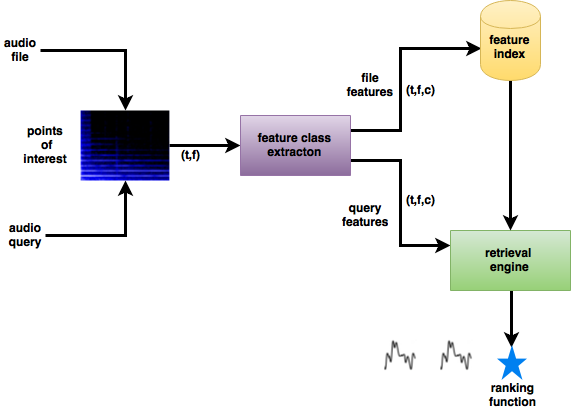
\includegraphics[scale=0.5]{Figures/qbe.png}
\decoRule
\caption[hypercube]{Typical illustration of Query-by-Example algorithm.}
\label{fig:qbe}
\end{figure}


One of the major drawback of the algorithm is insufficient invariance property. Additionally when the features are dense retrieval process gets slow on large corpora. Sometimes queries are long and queries require several second to execute which is not meaningful for realtime processing. One possible solution is to introduce segmentation instead of pont-of-interest which helps to achieve stronger invariance to timing variation and feature per segment will speedup the retrieval process. 

Digital Audio can be robustly segmented by correlating a kernal along the diagonal of self similarity matrix. A self similarity matrix is one which contains all possible pairwise similarity comparison between frames. Usually spectral data is used to calculate the inter-frame spectral similarity. When the matrix is normalized, the rows and columns sums to one and the diagonal represent the similarity of a frame with respect to itself. For instance the following shows image of a normalized self similarity matrix of a audio data which contains a repetitive phrase.
\begin{figure}[h]
\centering
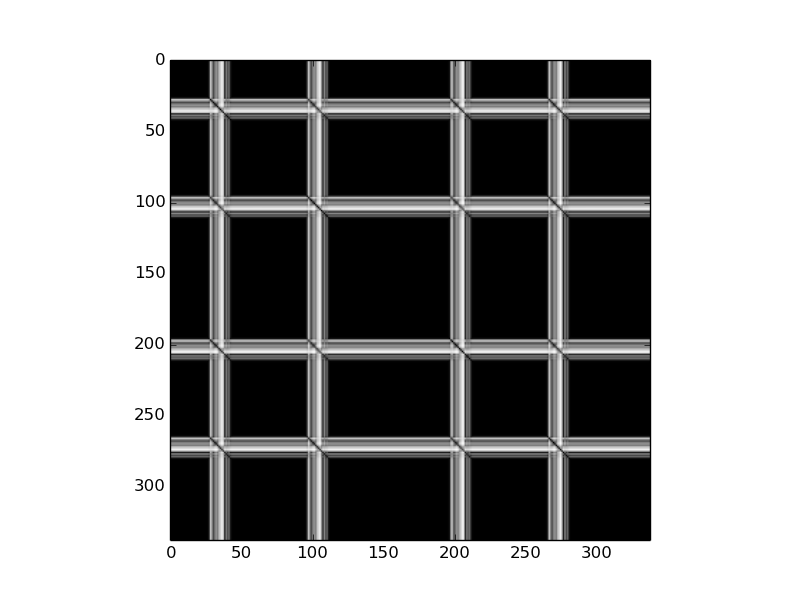
\includegraphics[scale=0.5]{Figures/self_similarity_1.png}
\decoRule
\caption[hypercube]{Image of a similarity matrix calculated from a audio data containing repeatative phrase.}
\label{fig:self_similarity}
\end{figure}

The similarity matrix can also be interpreted as markov chain where the $(i,j)$-th entry in the matrix represents the probability of  in the probability of transiting from frame $i$ to $j$. The following figure illustrates the four-state markov chain representation of a self-similarity matrix containing 4 frames, the figure also illustrates the transition matrix is upgraded to its $n$-th power and it's corresponding image:

\begin{figure}[h]
\centering
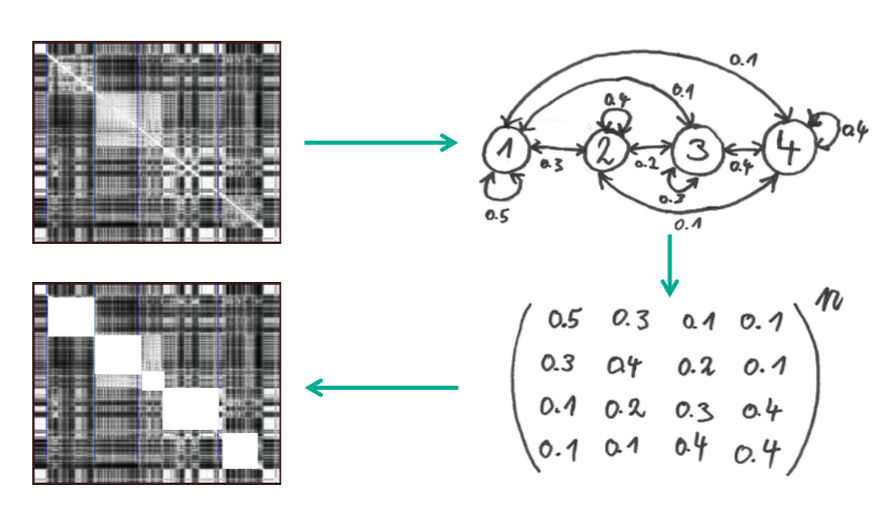
\includegraphics[scale=0.5]{Figures/markov.png}
\decoRule
\caption[hypercube]{Markov chain representation of self similarity matrix, and $n$-th power of the transition matrix.}
\label{fig:self_similarity}
\end{figure}



One can be more interested to calculate the projection of the self similarity matrix to an subspace and then use the projection for the segmentation. Which brings out the main problem of the thesis. The subspace holds the properties of a special polytope: Birkhoff polytope. Birkhoff polytope is matrix  whose all componants are non-negative real numbers and rows and columns sum to zero. The definition and properties of the birkhoff polytope has been described more elaborately in chapter \ref{chptr:birkhoff_polytope}. So far, no similar case has been found where a method specific to this application to calculate projection of self-similarity matrix to birkhoff polytope has been developed.

So the goal of the thesis is to develop a framework which can be used for audio segmentation. More specifically, a framework which can construct self-similarity matrix and calculate it's projection to the birkhoff polytope. It is required that, the method should be fast enough for realtime segmentation. In the next couple of sections problement and how the problem is formulated has been described.
 
\section{Problem Statement}

We would like to compute euclidian of a matrix $X$. So our goal is to compute the projection of $x^o$ to the Birkhoff Polytope with respect to the Euclidian Norm.

More precisely $\hat{X}$ can be written as minimiser:
\begin{equation}
\begin{aligned}
& \hat{X} = argmin \parallel \mathbf{X-X^o} \parallel _2\\
& \text{Subject to,}\\
& & \forall _{i,j} &\geq 0 \\
& & \sum_{i} x_{ij}&=1 \\
& & \sum_{j} x_{ij}&=1
\end{aligned}
\label{eqn:problem_statement}
\end{equation}

\section{Formulation of the Pronlem}
Given two polytopes $P$ and $Q$, defined by a total $k$ vertices in $d$ dimensional space. Find two points $p \in P$ anf $q \in Q$ with smalles euclidian distance. Wolfe addresed a special case where one polytope is defined by a single point. Murty and Fathi studied that polytope distance problem fits into the Quadratic Programming framework.\\
The quadratic programming can be formulated mathematically as-\\

Assume $X \in R^n$. Both x and d are column vector with n elements and $A$ is symmetric $\textbf{n} \times \textbf{n} $ matrix. Then,\\

\begin{equation}
\begin{aligned}
\underset{X}{\text{minimize}} \quad \frac{1}{2}X^\mathsf{T} PX+X^\mathsf{T}d\\
\text{subject to} \quad \\
a_i^\mathsf{T}x =b_i & & i\in \textrm{Equality Constraint}\\
a_j^\mathsf{T}x \geq b_j & & j\in \textrm{Equality Constraint}\\
\end{aligned}
\label{eqn:problem_formulation_1}
\end{equation}
 


To solve the problem in a qudratic programming appraoch it is required to identify the peremeters $P,d$, Inequality constraints and Equality Constraint. Now, From \ref{eqn:problem_statement}, it is found that
\begin{equation}
\begin{aligned}
\lVert {X-X_o} \rVert & = (X-X_o)^\mathsf{T}(X-X_o)\\
& = X^\mathsf{T}X-2X^{\mathsf{T}}X_o+X_o^{\mathsf{T}}X^o
\end{aligned}
\label{eqn:problem_formulation_2}
\end{equation}

If the variables of standard quadratic equation has been mapped with \ref{eqn:problem_formulation_2}, it is found that:
\begin{equation}
d=-2X_o \textrm{ column matrix of dimension }n^2\times 1
\end{equation}
\[P= 2\times
\begin{array}{c}
    \begin{bmatrix}
        1 & 0 & \cdots & 0\\
        0 & 1 & \cdots & 0\\
        \vdots & \vdots & \ddots & \vdots\\
        0 & 0 & \cdots & 1\\
    \end{bmatrix}\\
    n^2\times n^2
\end{array}
\]
In-Equality constraints:\\
\[G= -1 \times
\begin{array}{c}
    \begin{bmatrix}
        1 & 0 & \cdots & 0\\
        0 & 1 & \cdots & 0\\
        \vdots & \vdots & \ddots & \vdots\\
        0 & 0 & \cdots & 1\\
    \end{bmatrix}\\
    n^2\times n^2
\end{array}
\]
\\
\[h=
\begin{array}{c}
    \begin{bmatrix}
        0 \\
        0 \\
        \vdots\\
        0 \\
    \end{bmatrix}\\
    n^2\times 1
\end{array}
\]

Equality constraints:
































